\chapter{Concept Generation and Design Evaluation}\label{ch:design}
This chapter generates alternative concepts for each part of the system, evaluates
them against stated criteria, and describes the selected design. It defines the
evaluation criteria (Section~\ref{sec:criteria}), generates and assesses the
detector concepts (Section~\ref{sec:detector}) and the system concepts
(Section~\ref{sec:sysconcepts}), presents the selected architecture
(Section~\ref{sec:architecture}), discusses pre-processing and host association
(Section~\ref{sec:preproc}), and closes with the realistic constraints, standards
and ethical considerations (Section~\ref{sec:realistic}).

%-----------------------------------------------------------------------------
\section{Evaluation Criteria}\label{sec:criteria}
Each concept was judged against the five criteria in Table~\ref{tab:criteria}.
They follow from the requirements of Chapter~\ref{ch:system}: the system must run
real models now, produce traceable results, support an operator, remain
explainable by its student contributors, and avoid claims the evidence does not
support.

\begin{table}[htbp]
\centering\tablesetup
\caption{Criteria used to evaluate design concepts.}
\label{tab:criteria}
\begin{tabularx}{\textwidth}{@{}lL{0.25\textwidth}Y@{}}
\toprule
ID & Criterion & Question asked of each concept\\
\midrule
C1 & Demonstrated compatibility & Has it been executed with a verified,
task-matched checkpoint?\\
C2 & Reproducibility & Can a run be repeated and traced to its code, weights and
settings?\\
C3 & Operator value & Does it give the operator clear, localized and honest
feedback?\\
C4 & Effort and explainability & Can the team build it in SDP~I and explain every
part?\\
C5 & Claim risk & Does it avoid results or capabilities that the evidence does not
yet support?\\
\bottomrule
\end{tabularx}
\end{table}

%-----------------------------------------------------------------------------
\section{Detector Concepts}\label{sec:detector}
The IEDXray authors supplied checkpoints for six detector families, each trained
for the device, generic-explosive and specific-explosive tasks. They cover the
main design families of Section~\ref{sec:background}: a one-stage detector
(YOLOv10-M), two-stage detectors (Faster R-CNN and Cascade R-CNN), set-prediction
transformers (DETR and the anti-overlapping variant AO-DETR) and an open-set,
text-conditioned detector (Grounding DINO)~\citep{takele2026iedxray}. All 18 files
were hashed and their metadata inspected without loading the models. The
inspection found task-pairing problems in several non-YOLO files, such as a
specific-task Faster R-CNN checkpoint whose stored class names disagree with its
configured class count, and DETR files that store 92 outputs without class names.
\projectrecord{docs/checkpoint-catalog.md}

Table~\ref{tab:detector-eval} rates the six families against the criteria. A
rating of $+$ means the criterion is satisfied on current evidence, $\circ$ that
it is partly satisfied or unknown, and $-$ that it is not satisfied. The ratings
are a qualitative design assessment based on the inspection record, not a
measured accuracy comparison.

\begin{table}[htbp]
\centering\tablesetup
\caption{Qualitative evaluation of the supplied detector families
($+$ satisfied, $\circ$ partial or unknown, $-$ not satisfied).}
\label{tab:detector-eval}
\begin{tabularx}{\textwidth}{@{}L{0.2\textwidth}cccccY@{}}
\toprule
Detector family & C1 & C2 & C3 & C4 & C5 & Basis\\
\midrule
YOLOv10-M & $+$ & $+$ & $+$ & $+$ & $+$ & All three tasks executed on CPU and
GPU; class maps inspected; no NMS step\\
Faster R-CNN & $-$ & $\circ$ & $+$ & $\circ$ & $-$ & Head and label mismatch in
the specific task; needs MMDetection\\
Cascade R-CNN & $-$ & $\circ$ & $+$ & $\circ$ & $\circ$ & Class ordering of the
specific task unverified; needs MMDetection\\
DETR & $-$ & $-$ & $+$ & $\circ$ & $-$ & 92 outputs with no stored class names\\
AO-DETR & $-$ & $\circ$ & $+$ & $-$ & $\circ$ & Requires custom modules and
mapping verification\\
Grounding DINO & $-$ & $\circ$ & $+$ & $-$ & $-$ & Text prompts and category
handling must be verified together\\
\bottomrule
\end{tabularx}
\end{table}

YOLOv10-M is the only family that satisfies every criterion and is therefore the
selected reference detector. The other families remain research comparisons; no
local result is claimed for them. This selection reflects implementation evidence
and does not imply that YOLOv10-M scores highest in the IEDXray benchmark.

%-----------------------------------------------------------------------------
\section{System Concepts}\label{sec:sysconcepts}
Table~\ref{tab:alternatives} lists the alternatives considered for the other
design decisions and the reason for each selection. Each decision is also
recorded in the project's decision log.
\projectrecord{docs/decisions.md}

\begin{table}[htbp]
\centering\tablesetup
\caption{System design alternatives and the selected concept.}
\label{tab:alternatives}
\begin{tabularx}{\textwidth}{@{}L{0.17\textwidth}L{0.24\textwidth}L{0.2\textwidth}Y@{}}
\toprule
Decision & Alternatives & Selected & Reason\\
\midrule
Pipeline layout & Full-image detection; host-crop cascade & Full-image detection
& Avoids losing threats when a host box is missed (C3, C5); association rule
remains open\\
Image input & Manual upload; watched folder; scanner SDK & Upload, watched folder
and replay & Reversible and needs no scanner access; an SDK requires an observed
hardware interface (C1, C5)\\
Execution boundary & Model in main environment; isolated runtime & Isolated
runtime & Keeps the locked CPU tools small and each task's runtime qualified
(C2, C4)\\
Application stack & Desktop wrapper; cloud service; local web app &
React/TypeScript front end with local FastAPI & Runs locally without uploading
scans; familiar tools (C3, C4)\\
Interface between parts & Ad-hoc outputs; versioned contract & Versioned JSON
contract & Separates empty, missing and failed results; testable (C2, C3)\\
Study initialization & Continue author checkpoint; general pre-training &
General pre-training & The author checkpoint may have seen the validation images
(C5)\\
\bottomrule
\end{tabularx}
\end{table}

%-----------------------------------------------------------------------------
\section{Selected Architecture}\label{sec:architecture}
Figure~\ref{fig:architecture} shows the selected architecture. The application
and the research engine live in separate repositories. The operator interface and
a local API handle interaction; the engine, pinned as a Git submodule, supplies the
contracts, the model catalogue and the inference tools. The selected model runs in
its own qualified environment, and the API validates every returned scan result
before the interface displays it. The research path, which trains and validates
new candidates, was qualified and executed on the HPC cluster for the generic
study of Section~
ef{sec:results}; its checkpoints are not yet loaded by the
application.
\projectrecord{docs/architecture.md}

\begin{figure}[htbp]\centering
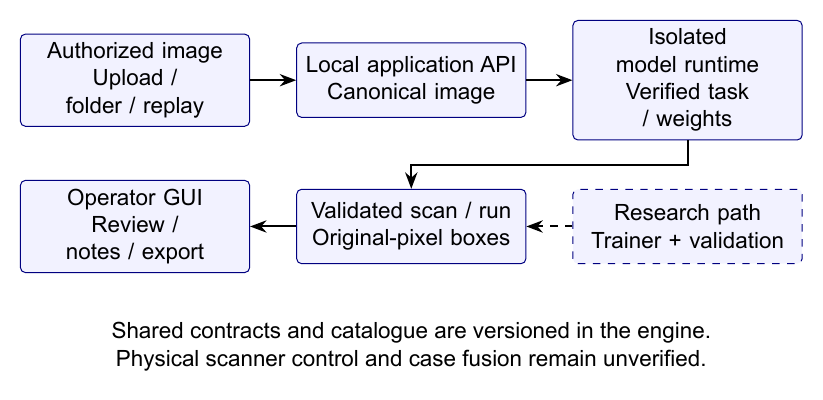
\includegraphics[width=\textwidth]{architecture.png}
\caption{Selected system architecture. Solid arrows show the implemented prototype
path; the dashed research path was executed on HPC for the generic study but is
not yet connected to the application.}
\label{fig:architecture}
\end{figure}

Two design rules keep the data consistent. First, the source image, its
canonically oriented copy and the original-coordinate predictions stay linked
throughout the pipeline. Second, operator viewing adjustments change only the
display and never become model pre-processing. Session history and saved evidence
also have different lifetimes: the visible session list may reset, while the
private run records remain.

%-----------------------------------------------------------------------------
\section{Pre-processing and Host Association}\label{sec:preproc}
The proposal asks for image enhancement such as noise reduction and contrast
adjustment. A filter applied before inference changes the input distribution that
the checkpoint was trained on, and may lower accuracy even if the image looks
clearer to a person. The design therefore applies only the checkpoint's own
normalization before inference and offers viewing adjustments, such as contrast, in
the display. Any enhancement before inference should be compared against an
identity reference under the validation protocol of Chapter~\ref{ch:theory}; no
benefit is claimed here.

The relation between a threat region and its host device was considered in two
forms. A \emph{host-crop cascade} first detects devices and then searches inside
each crop, which removes background but loses any threat whose host was missed;
it also needs rules for overlapping hosts, padding and regions crossing the crop
edge. \emph{Full-image detection} avoids that failure mode but still needs a
justified rule linking each threat to a host. The separate device and explosive
annotations of IEDXray do not decide between them, so the decision is left open
and the scan result records an explicit null association when the link is unknown.

%-----------------------------------------------------------------------------
\section{Realistic Constraints, Standards and Ethics}\label{sec:realistic}

\subsection{Realistic Constraints}
Table~\ref{tab:constraints} summarizes the constraints that shaped the design.

\begin{table}[htbp]
\centering\tablesetup
\caption{Realistic design constraints and the design response to each.}
\label{tab:constraints}
\begin{tabularx}{\textwidth}{@{}L{0.17\textwidth}YY@{}}
\toprule
Constraint & Situation & Design response\\
\midrule
Economic & Proposal budget of 1,000~AED; GPUs provided by the CVML laboratory &
Open-source software only; no paid services\\
Compute & HPC access with a time limit per job; runtime unknown at design time
& A bounded pilot before the search; measured study used 10~h of GPU time\\
Data & Limited real threat data; test split must stay untouched & Audit before
use; group-preserving partitions; new laboratory collection\\
Safety & Threat items are laboratory simulants; scanner operated in the
laboratory & Collection only under laboratory procedures\\
Privacy and security & Scans and credentials are sensitive & Local processing;
scans kept off the public repository\\
Time & One semester with five students & Small, explainable components with
clear interfaces\\
\bottomrule
\end{tabularx}
\end{table}

\subsection{Standards}
The design follows the COCO conventions for annotations and metrics and a versioned
JSON interface for interoperability between components~\citep{lin2014coco}. These
are technical conventions, not certification under aviation, radiation-safety or
security-screening standards; a deployed screening aid would require such
certification. The inspected IEDXray release contains processed RGB images rather
than the raw dual-energy signal, so material classes are not inferred from the
display colours.

\subsection{Ethics and Sustainability}
The main risks of the system are missed detections, operator over-reliance,
leakage of private data and misleading demonstrations. The design responds with
explicit error states, known misses kept in the record, provenance on every result
and the position of the system as an aid to a human operator. Laboratory work
follows the supervisor's scanner and safety procedures. On the computational side,
the study uses a measured pilot, a bounded number of trials and reuse of valid
results; no energy saving is claimed without measurement.

The selected design is implemented as described in Chapter~\ref{ch:implementation}.
